\begin{frame}[fragile]{Efficient, correct, safe, and secure}
\begin{minipage}{0.55\linewidth}
  \lstset{
    language=Jasmin,
    basicstyle=\footnotesize\ttfamily,
    escapechar=~~,
  }
  \begin{lstlisting}
fn memeq(reg u64 p q n) -> reg u64 {~~\loc{a00}~~
  reg u64 r one i;~~\loc{a01}~~
  r = 0;~~\loc{a02}~~
  one = 1;~~\loc{a03}~~
  i = 0;~~\loc{a04}~~
  while (i < n) {~~\loc{a05}~~
    if (r != 0) {~~\loc{a06}~~
      reg u64 a b;
      a = [p];~~\loc{a07}~~
      b = [q];~~\loc{a08}~~
      r = a != b ? one : r;~~\loc{a09}~~
      p += 8;~~\loc{a10}~~
      q += 8;~~\loc{a11}~~
    }~~\loc{a12}~~
    i = #INC(i);~~\loc{a13}~~
  }~~\loc{a14}~~
  return r;~~\loc{a15}~~
}~~\loc{a16}~~
  \end{lstlisting}
\end{minipage}\hfill%
\begin{minipage}{0.4\linewidth}
  \begin{uncoverenv}<2->
    \lstset{
      basicstyle=\scriptsize\ttfamily,
      escapechar=~~,
    }
    \begin{lstlisting}
~~\loc{b00}~~memeq:
  ~~\loc{b01}~~movq $0, %rax
  ~~\loc{b02}~~movq $1, %rcx
  ~~\loc{b03}~~movq $0, %r8
  ~~\loc{b04}~~jmp Lmemeq$1
~~\loc{b05}~~Lmemeq$2:
  ~~\loc{b06}~~cmpq $0, %rax
  ~~\loc{b07}~~je Lmemeq$3
  ~~\loc{b08}~~movq (%rdi), %r9
  ~~\loc{b09}~~movq (%rsi), %r10
  ~~\loc{b10}~~cmpq %r10, %r9
  ~~\loc{b11}~~cmovne %rcx, %rax
  ~~\loc{b12}~~addq $8, %rdi
  ~~\loc{b13}~~addq $8, %rsi
~~\loc{b14}~~Lmemeq$3:
  ~~\loc{b15}~~incq %r8
~~\loc{b16}~~Lmemeq$1:
  ~~\loc{b17}~~cmpq %rdx, %r8
  ~~\loc{b18}~~jb Lmemeq$2
  ~~\loc{b19}~~ret
    \end{lstlisting}
  \end{uncoverenv}
\end{minipage}

\begin{tikzpicture}[overlay, remember picture]
  \draw [->, visible on=<2-3>] (a02) -- (b01);
  \draw [->, visible on=<2-3>] (a03) -- (b02);
  \draw [->, visible on=<2-3>] (a04) -- (b03);
  \draw [->, visible on=<2-3>] (a07) -- (b08);
  \draw [->, visible on=<2-3>] (a08) -- (b09);
  \draw [->, visible on=<2-3>] (a09) -- (b10);
  \draw [->, visible on=<2-3>] (a09) -- (b11);
  \draw [->, visible on=<2-3>] (a10) -- (b12);
  \draw [->, visible on=<2-3>] (a11) -- (b13);
  \draw [->, visible on=<2>] (a13) -- (b15);

  \draw [->, dashed, Red, thick, visible on=<3>] (a13) -- (b15);

  \draw [->, densely dotted, thick, Green, visible on=<4>] (a00) -- (b00);
  \draw [->, densely dotted, thick, Green, visible on=<4>] (a15) -- (b19);

  \draw [->, Red, visible on=<4>] (a05) -- (b04);
  \draw [->, Red, visible on=<4>] (a05) -- (b05);
  \draw [->, Red, visible on=<4>] (a05) -- (b16);
  \draw [->, Red, visible on=<4>] (a05) -- (b17);
  \draw [->, Red, visible on=<4>] (a05) -- (b18);

  \draw [->, dashed, Blue, visible on=<4>] (a06) -- (b06);
  \draw [->, dashed, Blue, visible on=<4>] (a06) -- (b07);
  \draw [->, dashed, Blue, visible on=<4>] (a06) -- (b14);
\end{tikzpicture}%
\end{frame}

\begin{frame}{More online}
  \begin{center}
    \begin{figure}[t]
      \centering
      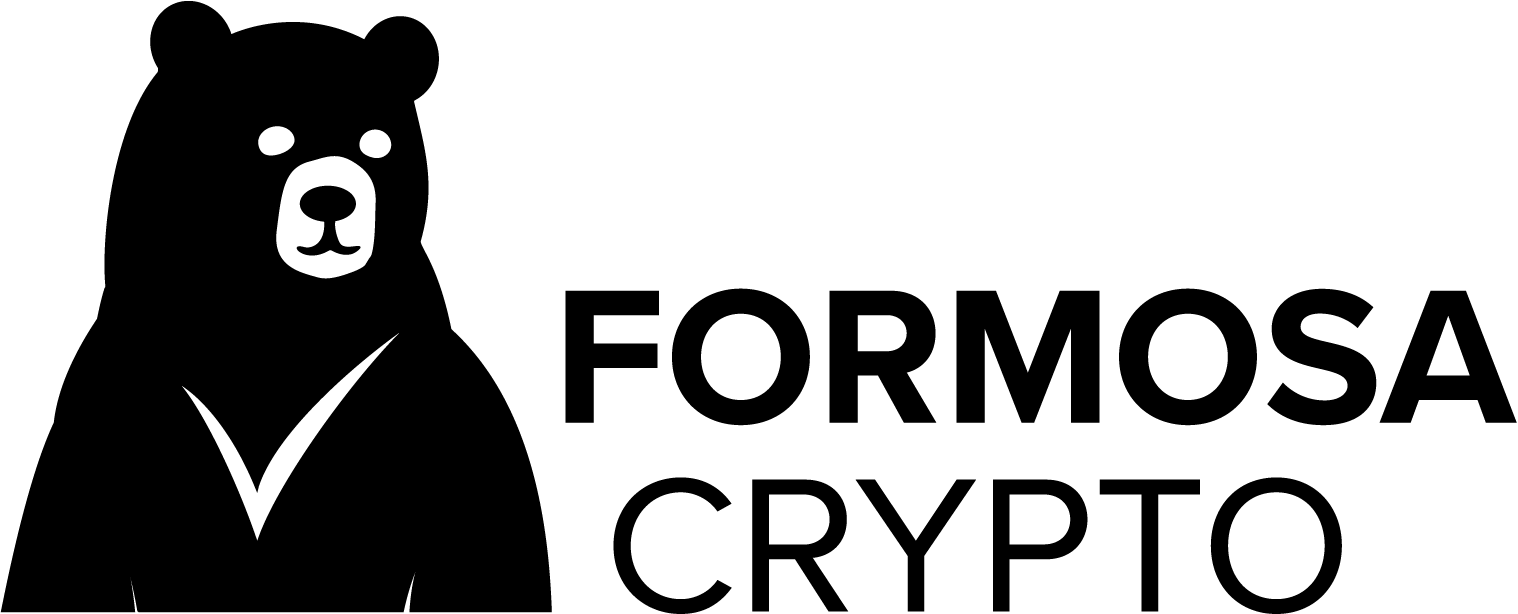
\includegraphics[width=0.4\textwidth]{formosa}
      \caption*{\Large \url{formosa-crypto.org}}
    \end{figure}
  \end{center}
  \vspace*{.5cm}
  \begin{itemize}
  \item[] \textbf{Jasmin:} \url{github.com/jasmin-lang/jasmin}
  \item[] \textbf{EasyCrypt specifications:}
    \url{github.com/formosa-crypto/crypto-specs}
  \item[] \textbf{Libjade:} \url{github.com/formosa-crypto/libjade}
  \end{itemize}
\end{frame}
